\documentclass{article}

\usepackage{graphicx}
\usepackage{tikz}
\usepackage{tikzsymbols}
\usetikzlibrary{calc,patterns,shapes.geometric}
\pagestyle{empty}
\usepackage[margin=0pt]{geometry}
\geometry{papersize={14in,12in}}

\def\centerarc[#1](#2)(#3:#4:#5){\draw[#1] ($(#2)+({#5*cos(#3)},{#5*sin(#3)})$) arc (#3:#4:#5);}

\begin{document}
	\begin{figure}
		\centering
		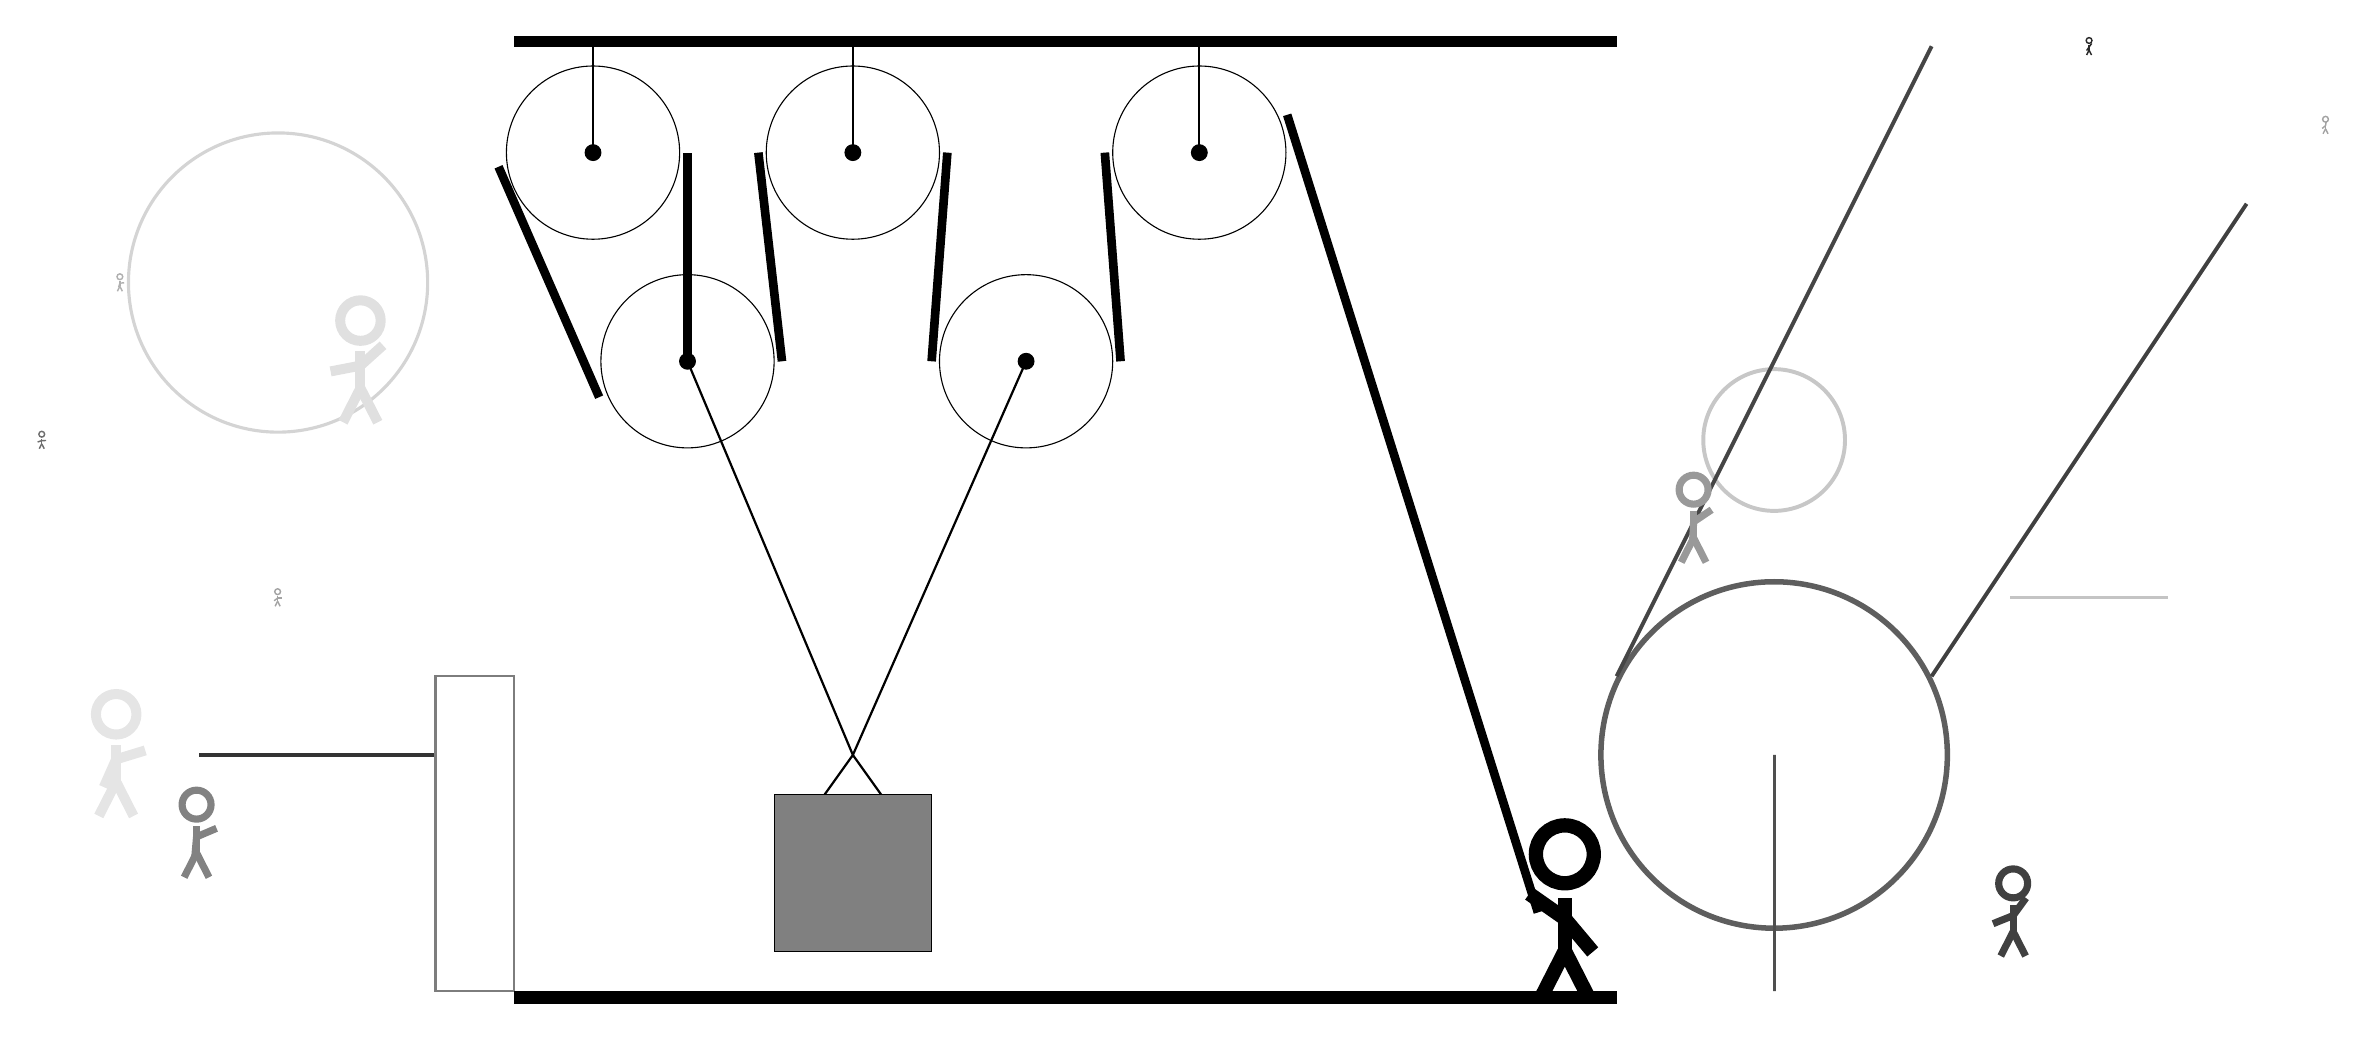
\begin{tikzpicture}
			%%%%% START %%%%%
			
			\draw[fill=black] (-2, 9) rectangle (12, 9.125);
			
			\draw (-1, 7.65) circle (1.1);
			\draw[fill=black] (-1, 7.65) circle (0.1);
			\draw[thick] (-1, 7.65) -- (-1, 9);
			
			\draw (2.3, 7.65) circle (1.1);
			\draw[fill=black] (2.3, 7.65) circle (0.1);
			\draw[thick] (2.3, 7.65) -- (2.3, 9);
			
			\draw (6.7, 7.65) circle (1.1);
			\draw[fill=black] (6.7, 7.65) circle (0.1);
			\draw[thick] (6.7, 7.65) -- (6.7, 9);
			
			\draw (0.2, 5) circle (1.1);
			\draw[fill=black] (0.2, 5) circle (0.1);
			
			\draw (4.5, 5) circle (1.1);
			\draw[fill=black] (4.5, 5) circle (0.1);
			
			\draw[thick] (0.2, 5) -- (2.3, 0)  -- (4.5, 5);
			\draw[thick]  (1.8, -0.7) -- (2.3, 0) -- (2.8, -0.7);
			\draw[fill=black!50] (1.3, -0.5) rectangle (3.3, -2.5);
			
			\draw[line width=1.1mm] (0.2, 5) -- (0.2, 7.65);
			\centerarc[line width=1.1mm](-1, 7.65)(0:200:1.2000000000000002);
			\draw[line width=1.1mm] (-2.2, 7.47) -- (-0.922, 4.544);
			\centerarc[line width=1.1mm](0.2, 5)(200:360:1.2000000000000002);
			\draw[line width=1.1mm](1.4, 5) -- (1.1, 7.65);
			\centerarc[line width=1.1mm](2.3, 7.65)(0:180:1.2000000000000002);
			\draw[line width=1.1mm] (3.5, 7.65) -- (3.3, 5);
			\centerarc[line width=1.1mm](4.5, 5)(180:360:1.2000000000000002);
			\draw[line width=1.1mm] (5.7, 5) -- (5.5, 7.65);
			\centerarc[line width=1.1mm](6.7, 7.65)(20:180:1.2000000000000002);
			\draw[line width=1.1mm](7.816, 8.13)  -- (11, -2);
			
			\node[line width=0.2mm, color=black!84] at (18, 9) {\Strichmaxerl[1][55][53]};
			
			\draw[line width=0.5mm, color=black!80](-3, 0) -- (-6, 0);
			\draw[line width=0.3mm, color=black!51] (-3, 1) rectangle (-2, -3);
			\node[line width=0.2mm, color=black!49] at (-6, -1) {\Strichmaxerl[5][85][23]};
			
			\node[line width=0.2mm, color=black!57] at (-8, 4) {\Strichmaxerl[1][18][2]};
			\draw [line width=0.7mm, color=black!63](14, 0) circle (2.2);
			
			\node[line width=0.6mm, color=black!75] at (17, -2) {\Strichmaxerl[5][22][54]};
			\node[line width=0.7mm, color=black!31] at (-7, 6) {\Strichmaxerl[1][73][5]};
			\draw[line width=0.5mm, color=black!75](16, 1) -- (20, 7);
			\draw[line width=0.5mm, color=black!23](17, 2) -- (19, 2);
			
			\node[line width=0.3mm, color=black!36] at (-5, 2) {\Strichmaxerl[1][37][0]};
			\draw [line width=0.5mm, color=black!22](14, 4) circle (0.9);
			\draw[line width=0.5mm, color=black!73](16, 9) -- (12, 1);
			\node[line width=0.5mm, color=black!36] at (21, 8) {\Strichmaxerl[1][40][80]};
			\draw [line width=0.4mm, color=black!17](-5, 6) circle (1.9);
			\node[line width=0.5mm, color=black!40] at (13, 3) {\Strichmaxerl[5][87][34]};
			
			\node[line width=0.7mm, color=black!10] at (-7, 0) {\Strichmaxerl[7][66][17]};
			\draw[line width=0.4mm, color=black!69] (14, -3) rectangle (14, 0);
			\node[line width=0.6mm, color=black!12] at (-4, 5) {\Strichmaxerl[7][11][42]};
			
			
			\node at (11.3, -2) {\Strichmaxerl[10][-35][-50]};
			
			\draw[fill=black] (-2, -3) rectangle (12, -3.15);
			
			%%%%% END %%%%%
		\end{tikzpicture}
	\end{figure}	
\end{document}